\documentclass{report}
\usepackage{geometry}
\usepackage{graphicx}
% Define a custom environment with reduced margins
\newenvironment{narrowmargins}{
    \newgeometry{top=1in, bottom=1in, left=0.5in, right=0.5in}
}{\restoregeometry}


\title{Implementation Report Analysis}
\author{Vivado}
\date{\today}

\begin{document}
\maketitle

\chapter{Introduction}

This document is an analysis of the implementation report generated by Vivado for the \texttt{top} module. The report is generated after the implementation process is completed. The report contains information about the resources used by the design, the timing constraints, and the timing performance of the design. The report is used to analyze the design and to identify any potential issues that may need to be addressed.

\chapter{Resource Utilization}

The resource utilization section of the report provides information about the resources used by the design. This includes information about the number of LUTs, FFs, BRAMs, and DSPs used by the design. The resource utilization section also provides information about the number of IOBs used by the design.

\section{Common Resource Types}
Here are some common resource types used in FPGA designs and Verilog codes that utilizes these resources:
\subsection{LUTs}
LUTs (Look-Up Tables) are fundamental building blocks in FPGA designs. They are used to implement combinational logic functions. Each LUT has a fixed number of inputs and a single output. The Verilog code snippet below shows an example of a 2-input LUT implementation:

\begin{verbatim}
module lut2 (input wire a, b, output wire y);
    assign y = a & b;
endmodule
\end{verbatim}

\subsection{FFs}
FFs (Flip-Flops) are sequential elements used to store and propagate data in FPGA designs. They are commonly used to implement registers and memory elements. The Verilog code snippet below shows an example of a D flip-flop implementation:

\begin{verbatim}
module dff (input wire clk, reset, input wire d, output reg q);
    always @(posedge clk or posedge reset)
        if (reset)
            q <= 1'b0;
        else
            q <= d;
endmodule
\end{verbatim}

\subsection{BRAMs}
BRAMs (Block RAMs) are memory elements in FPGA designs. They provide large storage capacity and high-speed access. They can be coded into fpga, or The Verilog code snippet below shows an example of a simple dual-port RAM implementation:

\begin{verbatim}
module dual_port_ram (input wire clk, input wire [7:0] addr_a, addr_b,
                      input wire [7:0] data_a, data_b,
                      input wire we_a, we_b,
                      output reg [7:0] q_a, q_b);
    reg [7:0] mem [0:255];
    
    always @(posedge clk)
        if (we_a)
            mem[addr_a] <= data_a;
    
    always @(posedge clk)
        if (we_b)
            mem[addr_b] <= data_b;
    
    always @(*)
        q_a = mem[addr_a];
        q_b = mem[addr_b];
endmodule
\end{verbatim}


\subsection{DSPs}
DSPs (Digital Signal Processors) are specialized hardware blocks in FPGA designs used for high-performance signal processing operations. They are commonly used in applications such as image and audio processing. The Verilog code snippet below shows an example of a simple multiplier using DSP blocks:

\begin{verbatim}
module multiplier (input wire [9:0] a, b, output wire [19:0] result);
    assign result = a * b;
endmodule
\end{verbatim}
\begin{figure}[ht]
    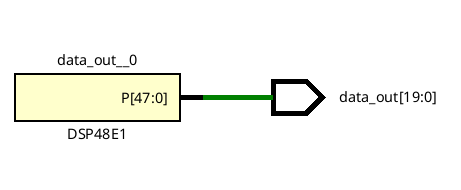
\includegraphics[width=0.4\linewidth]{images/dsp.png}
    \centering
    \caption{DSP Block Implemented}
    \label{fig:dsp}
\end{figure}

*For Basys3 Vivado prefers to use dsp blocks 10 and more bits multiplication. For 9 bits and less, it uses LUTs and FFs, but adding \texttt{(* use\_dsp = "yes" *)} to the module can force Vivado to DSP for arithmetic operations.

\subsection{IOBs}
IOBs (Input/Output Blocks) are used to interface the FPGA design with external devices. They provide the necessary logic to drive and receive signals from the external world. The Verilog code snippet below shows an example of an IOB implementation for a simple GPIO (General Purpose Input/Output) interface:

\begin{verbatim}
module gpio (input wire clk, input wire reset, input wire [7:0] data_in,
             output wire [7:0] data_out, inout wire [7:0] io_pins);
    reg [7:0] internal_reg;
    
    always @(posedge clk or posedge reset)
        if (reset)
            internal_reg <= 8'b0;
        else
            internal_reg <= data_in;
    
    assign data_out = internal_reg;
    assign io_pins = internal_reg;
endmodule
\end{verbatim}

\section{Resource Utilization Report}

The resource utilization report provides information about how many of these components are available in the FPGA and how many are used by your design. It helps you understand how efficiently your design is utilizing the available resources and whether any adjustments or optimizations are needed.

\paragraph{There are 8 parts in the resource utilization report.}
\begin{enumerate}
    \item Slice Logic: How many LUTs and FFs are used in the design. How many of LUTs are used as Logic or Memory and how many of FFs are used as Registers or Latches.
    \item Slice Logic Distribution: How the LUTs and FFs are distributed across the slices.
    \item Memory: Usage report of build in memory blocks. There can be different types for different fpga families.
    \item DSPs: Usage report of DSP blocks.
    \item IOs
    \item BUFG/BUFGCTRL (Clocking): Usage report of clocking resources.
    \item Specific Feature: Usage report of specific featured blocks of the fpga card.
    \item Primitive: How many of each primitive type are utilized in your design. A more detailed report of the sources mentioned in the other tables used in the design. It doesn't give the utilization ratio.
\end{enumerate}

Example scenarios to chose which part to look at:
\begin{itemize}
    \item If you wanted to know exactly how many flip-flops or LUTs of a particular configuration (like FDRE for a flip-flop with enable) were used, you would consult the Primitive Types Report.
    \item If the design is using a lot of memory resources as LUT, you may want to look at the Memory section to see if there are any optimizations that can be made.
    \item If the design is using a lot math operations, you may want to look at the DSP and LUT section to see if the design is close to the limits.
    \item \textbf{***The synthesis tool might not be able to utilize the desing as desired. A different block of fpga can be used to implement your design. For example a buffer can be utilized in BRAMs, LUTRAMs, or FFs. Simple changes in your design can make implementation tool to chose a different resource. ***} 
\end{itemize}
An example table from resource utilization report for the \texttt{top} module is shown below:


\begin{verbatim}
    8. Primitives
    -------------
    
    +----------+------+---------------------+
    | Ref Name | Used | Functional Category |
    +----------+------+---------------------+
    | FDRE     |  178 |        Flop & Latch |
    | LUT6     |   79 |                 LUT |
    | LUT4     |   48 |                 LUT |
    | LUT5     |   22 |                 LUT |
    | LUT2     |   21 |                 LUT |
    | LUT3     |   18 |                 LUT |
    | CARRY4   |   11 |          CarryLogic |
    | FDSE     |   10 |        Flop & Latch |
    | OBUF     |    7 |                  IO |
    | RAMB18E1 |    4 |        Block Memory |
    | IBUF     |    3 |                  IO |
    | LUT1     |    2 |                 LUT |
    | BUFG     |    2 |               Clock |
    +----------+------+---------------------+
    
\end{verbatim}

General file names for this report are \texttt{Module\_Name\_utilization\_routed.rpt} or \texttt{Module\_Name\_utilization\_placed.rpt}.

\chapter{Power Analysis}
Power analysis is an important aspect of FPGA design as it helps in understanding the power consumption of the implemented design. By analyzing the power utilization, we can optimize the design to reduce power consumption and improve overall efficiency. Power analysis provides insights into the power consumption of different components in the design, such as LUTs, FFs, BRAMs, DSPs, and IOBs. It also helps in identifying any potential power-related issues that may need to be addressed. In this section, we will explore the power utilization of the \texttt{top} module and analyze the power consumption of various components in the design.

\section{Power Utilization Report}
The power utilization report provides information about the power consumption of different components in the design. It includes details about the dynamic power, static power, and total power consumption of the design. 
There are 3 parts in the power utilization report. The content of the report may vary depending on the FPGA family and the tool used. \paragraph{However, The first two table \(1.1\ and\  1.2\) and the last table \(3.1\) are the most useful table for power analysis.} 
\begin{itemize}
    \item 1.1 Power Summary: This table provides an overview of the power consumption of the design. It includes information about the dynamic power, static power, dynamic power, and total power consumption of the design. It also provides details about constraints (if you set).
    \item 1.2 Power by Component: This table provides detailed information about the power consumption of different components in the design. It includes information about the power consumption of LUTs, FFs, BRAMs, DSPs, and IOBs. It helps in understanding the power consumption of different components and optimizing the design to reduce power consumption.
    \item 3.1 Power by Hierarchy: This table provides a hierarchical view of the power consumption of the design. It includes information about the power consumption of different modules in the design and helps in identifying the power consumption of individual modules.
\end{itemize}

\subsection{Power Summary (1.1)}
An example table from power utilization report for the \texttt{top} module is shown below:

\begin{verbatim}
    +--------------------------+--------------+
| Total On-Chip Power (W)  | 0.082        |
| Design Power Budget (W)  | Unspecified* |
| Power Budget Margin (W)  | NA           |
| Dynamic (W)              | 0.010        |
| Device Static (W)        | 0.072        |
| Effective TJA (C/W)      | 5.0          |
| Max Ambient (C)          | 84.6         |
| Junction Temperature (C) | 25.4         |
| Confidence Level         | Medium       |
| Setting File             | ---          |
| Simulation Activity File | ---          |
| Design Nets Matched      | NA           |
+--------------------------+--------------+
\end{verbatim}

An explanation of the fields and tips about some fields in the table is as follows:
\begin{itemize}
    \item Total On-Chip Power (W): The total power consumption of the design on the FPGA chip.
    \item Design Power Budget (W): The specified power budget for the design. \textbf{If you set a power budget, you can compare the actual power consumption with the specified power budget to ensure that the design meets the power requirements. If you need to run on battery power, this might be important.}
    \item Power Budget Margin (W): The margin between the actual power consumption and the specified power budget.
    \item Dynamic (W): The dynamic power consumption of the design. \textbf{High dynamic power drawn when performance required. It is best to keep power drawn low when not required. For example, if your design uses multiple modules used as needed, you can disable their clocks when they are not used. This should reduce dynamic power.}
    \item Device Static (W): The static power consumption of the FPGA device. \textbf{This should be reduced to keep power consumption and temperature low. Power gating can be used to reduce static power. This is not available for all FPGAs please research.}
    \item Effective TJA (C/W): The thermal junction-to-ambient resistance of the FPGA device.
    \item Max Ambient (C): The maximum ambient temperature for the design.
    \item Junction Temperature (C): The junction temperature of the FPGA device.
    \item Confidence Level: The confidence level of the power analysis results. This depends on the user specifications. \textbf{If you want a more accurate result, you can increase the confidence level by setting io and clock activity using GUI or constraints file.}
    \item Setting File: The settings file used for the power analysis.
    \item Simulation Activity File: The simulation activity file used for the power analysis.
    \item Design Nets Matched: The number of design nets matched during the power analysis.
\end{itemize}

\subsection{Power by Component (1.2)}
An example table from power utilization report for the \texttt{top} module is shown below:
\begin{verbatim}
+----------------+-----------+----------+-----------+-----------------+
| On-Chip        | Power (W) | Used     | Available | Utilization (%) |
+----------------+-----------+----------+-----------+-----------------+
| Clocks         |     0.001 |        5 |       --- |             --- |
| Slice Logic    |    <0.001 |      406 |       --- |             --- |
|   LUT as Logic |    <0.001 |      164 |     20800 |            0.79 |
|   Register     |    <0.001 |      188 |     41600 |            0.45 |
|   CARRY4       |    <0.001 |       11 |      8150 |            0.13 |
|   Others       |     0.000 |       17 |       --- |             --- |
| Signals        |    <0.001 |      363 |       --- |             --- |
| Block RAM      |    <0.001 |        2 |        50 |            4.00 |
| I/O            |     0.007 |       10 |       106 |            9.43 |
| Static Power   |     0.072 |          |           |                 |
| Total          |     0.082 |          |           |                 |
+----------------+-----------+----------+-----------+-----------------+
\end{verbatim}
Using this table and information from the previous section, you can analyze the power consumption of different components in the design and identify areas where power optimization is needed. For example, if the design is using a large number of LUTs, you can optimize the design to reduce the number of LUTs used and reduce power consumption. Similarly, if the design is using a large number of a component, and if it is more efficient to use other blocks you can force to use other blocks for your design.

\subsection{Power by Hierarchy (3.1)}
An example table from power utilization report for the \texttt{top} module is shown below:
\begin{verbatim}
+---------------+-----------+
| Name          | Power (W) |
+---------------+-----------+
| MemController |     0.010 |
+---------------+-----------+
\end{verbatim}
This table is not a great example,but if yours include your sub modules you can analyze the power consumption of different modules in the design and identify areas where power optimization is needed. For example, if a particular module is consuming a large amount of power, you can optimize that module to reduce power consumption.

\chapter{Methodology Warnings}
The methodology warnings section of the report provides information about any potential issues or warnings that may need to be addressed. This section includes information about the timing constraints, clock constraints, and other design constraints that may impact the performance of the design. The methodology warnings section helps in identifying any potential issues that may need to be addressed to improve the performance of the design.

\section{Methodology Warnings Report}
Example issues from methodology warnings report for the \texttt{top} module is shown below:
\begin{verbatim}
    [Timing 38-282] The design failed to meet the timing requirements. 
    Please see the timing summary report for details on the timing violations.

    [Place 30-58] IO placement is not user specified.

    TIMING-18#1 Warning
    Missing input or output delay  
    An input delay is missing on reset relative to the rising and/or falling clock edge(s) 
    of sys_clk_pin.
    Related violations: <none>
\end{verbatim}
Some of this issues are about the constraints that you did not set. Some can be ignored if you are confident about timing latency of those pins. However, if you are not sure about the latency of the pins, you can set the constraints for those pins. Then if you get timing failed warning, your system will be high probably not working as desired stably. IO placement is more important, there might be bitstream write issues even if it is implemented. Also, if the tool can place as it wants, the design may not function as desired on the device. You can check the io placement in \texttt{Module\_Name\_io\_placed.rpt} file.

\chapter{Timing Analysis}
The timing analysis section of the report provides information about the timing performance of the design. This includes information about the clock constraints, setup and hold times, clock-to-q delays, and other timing parameters that impact the performance of the design. The timing analysis section helps in identifying any potential timing issues that may need to be addressed to improve the performance of the design. This is the most complex and important part of the report.
\section{Definitions and Explanations}
These are some common terms used in the timing analysis report in order to understand the report better:
\begin{itemize}
    \item \textbf{Setup Time:} The amount of time the input signal must be stable before the active edge of the clock signal. If the input signal changes too close to the active edge of the clock signal, the flip-flop may not capture the correct value.
    \item \textbf{Hold Time:} The amount of time the input signal must be stable after the active edge of the clock signal. If the input signal changes too soon after the active edge of the clock signal, the flip-flop may not capture the correct value.
    \item \textbf{Slack:} The slack is the amount of time by which the actual timing of the design exceeds the required timing. A positive slack indicates that the design meets the timing requirements, while a negative slack indicates that the design fails to meet the timing requirements.
    \item \textbf{Clock-to-Q Delay:} The amount of time it takes for the output signal to change after the active edge of the clock signal. This is the delay through the flip-flop.
    \item \textbf{Clock Skew:} The difference in arrival times of the clock signal at different flip-flops. Clock skew can cause timing violations if the clock signal arrives at different flip-flops at different times.
    \item \textbf{Clock Uncertainty:} The amount of uncertainty in the clock signal arrival time. Clock uncertainty can cause timing violations if the clock signal arrives at different flip-flops at different times.
    \item \textbf{Critical Path:} The path in the design with the longest delay. The critical path determines the maximum clock frequency of the design.
    \item \textbf{Timing Violation:} A timing violation occurs when the design fails to meet the timing requirements specified in the constraints file. Timing violations can cause the design to malfunction or fail to meet the desired performance.
    \item \textbf{Clock Domain Crossing:} Clock domain crossing occurs when signals from one clock domain are transferred to another clock domain. Clock domain crossing can cause timing violations if the signals are not synchronized properly.
    \item \textbf{False Path:} A false path is a path in the design that is not required to meet the timing requirements. False paths are ignored by the timing analysis tool to reduce the analysis time.
    \item \textbf{TNS: } Total Negative Slack. The sum of all negative slack values in the design.
    \item \textbf{WNS: } Worst Negative Slack. The worst negative slack value in the design.
    \item \textbf{THS: } Total Hold Slack. The sum of all hold slack values in the design.
    \item \textbf{WHS: } Worst Hold Slack. The worst hold slack value in the design.
    \item \textbf{WPWS: } Worst Pulse Width Slack. The worst pulse width slack value in the design.
    \item \textbf{Data Path Delay: } The amount of time it takes for the data signal to propagate through the combinational logic in the design. Data path delay is a critical parameter that impacts the overall performance of the design.
    \item \textbf{System Jitter: } The amount of variation in the clock signal arrival time. System jitter can cause timing violations if the clock signal arrives at different flip-flops at different times.
    \item \textbf{Input Jitter: } The amount of variation in the input signal arrival time. Input jitter can cause timing violations if the input signal changes too close to the active edge of the clock signal.
\end{itemize}
\section{Calculation of Slack}
The slack is calculated as follows:
\begin{verbatim}
    Time Avaliable for Data Setup = Clock Period - Data Path Delay
    Setup Slack = (Clock Period) - (Time Avaliable for Data Setup)

    Time Avaliable for Data Hold = Data Change Time after Clock Edge
    Hold Slack = Time Avaliable for Data Hold - Hold Time

    Time Required = Time Required for Pulse to be High 
    Actual Pulse Width = Time that the Pulse is High
    Pulse Width Slack = Actual Pulse Width - Time Required
\end{verbatim}
\section{Timing Analysis Report}
The timing analysis doesn't have expilicit sections like the other reports. It is a long report that includes all the timing information of the design. However, we can break it down into 4 parts:

\subsection{Timing Checks}
At the start of the timing analysis report, there is a summary of the timing checks. These checks make sure that an accurate timing report is produced. The summary provides timing warnings for your design. This suggestions might be useful to fix the timing issues.
An example from the timing analysis report for the \texttt{top} module is shown below:
\begin{verbatim}
    Table of Contents
    -----------------
    1. checking no_clock (0)
    2. checking constant_clock (0)
    3. checking pulse_width_clock (0)
    4. checking unconstrained_internal_endpoints (0)
    5. checking no_input_delay (2)
    6. checking no_output_delay (6)
    7. checking multiple_clock (0)
    8. checking generated_clocks (0)
    9. checking loops (0)
    10. checking partial_input_delay (0)
    11. checking partial_output_delay (0)
    12. checking latch_loops (0)
    
    1. checking no_clock (0)
    ------------------------
     There are 0 register/latch pins with no clock.
    
    
    2. checking constant_clock (0)
    ------------------------------
     There are 0 register/latch pins with constant_clock.
    
    
    3. checking pulse_width_clock (0)
    ---------------------------------
     There are 0 register/latch pins which need pulse_width check
    
    
    4. checking unconstrained_internal_endpoints (0)
    ------------------------------------------------
     There are 0 pins that are not constrained for maximum delay.
    
     There are 0 pins that are not constrained for maximum delay due to constant clock.
    
    
    5. checking no_input_delay (2)
    ------------------------------
     There are 2 input ports with no input delay specified. (HIGH)
    
     There are 0 input ports with no input delay but user has a false path constraint.
    
    
    6. checking no_output_delay (6)
    -------------------------------
     There are 6 ports with no output delay specified. (HIGH)
    
     There are 0 ports with no output delay but user has a false path constraint
    
     There are 0 ports with no output delay but with a timing clock defined on it 
     or propagating through it
    
    
    7. checking multiple_clock (0)
    ------------------------------
     There are 0 register/latch pins with multiple clocks.
    
    
    8. checking generated_clocks (0)
    --------------------------------
     There are 0 generated clocks that are not connected to a clock source.
    
    
    9. checking loops (0)
    ---------------------
     There are 0 combinational loops in the design.
    
    
    10. checking partial_input_delay (0)
    ------------------------------------
     There are 0 input ports with partial input delay specified.
    
    
    11. checking partial_output_delay (0)
    -------------------------------------
     There are 0 ports with partial output delay specified.
    
    
    12. checking latch_loops (0)
    ----------------------------
     There are 0 combinational latch loops in the design through latch input
\end{verbatim}
Using this information, you can identify any potential timing issues in the design and take appropriate actions to address them. For example, if there are input ports with no input delay specified, you can set the input delay constraints to ensure that the design meets the timing requirements.
If the design has a negative slack, the input delay that is not specified might be causing this result.
This warnings effect the detailed design timing summary which comes after.

\subsection{Design Timing Summary}
After the checks, there is a timing report of the whole module.
An example from the timing analysis report for this part is shown below:

\begin{verbatim}
----------------------------------------------------------------------------------
| Design Timing Summary                                                          |
| ---------------------                                                          |
----------------------------------------------------------------------------------

WNS(ns)      TNS(ns)  TNS Failing Endpoints  TNS Total Endpoints      WHS(ns)      
-------      -------  ---------------------  -------------------      -------
3.864        0.000                      0                  561        0.058

THS(ns)  THS Failing Endpoints  THS Total Endpoints     WPWS(ns)     TPWS(ns)  
-------  ---------------------  -------------------     --------     -------- 
0.000                      0                  561        4.500        0.000   

TPWS Failing Endpoints  TPWS Total Endpoints  
----------------------  --------------------
                     0                   198    
\end{verbatim}

The titles are already explained in the previous part. If there is no negative value or close to zero, the design is working as desired. If there is a negative value, you should check the detailed timing report to see which part of the design is causing the issue.
Hold times are close to zero, but they are how they are suppose to be as hold time is already a small value.

\subsection{Clock Timing Summary}
After the design timing summary, there is a clock timing summary. This part provides information about the clock constraints, slacks for each clock's own domain, slacks between clock domains, and clock uncertainty of the design. It helps in understanding the clock performance of the design and identifying any potential clock-related issues that may need to be addressed.
An example from the timing analysis report for this part is shown below:

\begin{verbatim}
    ------------------------------------------------------------------------------------------------
    | Clock Summary
    | -------------
    ------------------------------------------------------------------------------------------------
    
    Clock        Waveform(ns)           Period(ns)      Frequency(MHz)
    -----        ------------           ----------      --------------
    sys_clk_pin  {0.000 5.000}          10.000          100.000         
      rx_clk     {0.000 270.000}        540.000         1.852           
      tx_clk     {0.000 4340.000}       8680.000        0.115           
    
    
    ------------------------------------------------------------------------------------------------
    | Intra Clock Table
    | -----------------
    ------------------------------------------------------------------------------------------------
    
    Clock             WNS(ns)      TNS(ns)  TNS Failing Endpoints  TNS Total Endpoints
    -----             -------      -------  ---------------------  -------------------
    sys_clk_pin         4.227        0.000                      0                  445
    rx_clk            535.110        0.000                      0                   74
    tx_clk           8675.541        0.000                      0                   34
    
    WHS(ns)      THS(ns)  THS Failing Endpoints  THS Total Endpoints     WPWS(ns)
    -------      -------  ---------------------  -------------------     --------
      0.058        0.000                      0                  445        4.500
      0.177        0.000                      0                   74      269.500
      0.191        0.000                      0                   34     4339.500

    
    
    TPWS(ns)  TPWS Failing Endpoints  TPWS Total Endpoints  
    --------  ----------------------  --------------------  
       0.000                       0                   140  
       0.000                       0                    40
       0.000                       0                    18      
    
    
       ------------------------------------------------------------------------------------------------
    | Inter Clock Table
    | -----------------
    ------------------------------------------------------------------------------------------------
    
    From Clock    To Clock          WNS(ns)      TNS(ns)  TNS Failing Endpoints
    ----------    --------          -------      -------  ---------------------
    rx_clk        sys_clk_pin         3.864        0.000                      0
    tx_clk        sys_clk_pin         5.181        0.000                      0
    sys_clk_pin   tx_clk              6.771        0.000                      0

    TNS Total Endpoints      WHS(ns)      THS(ns)  THS Failing Endpoints
    -------------------      -------      -------  ---------------------
                     69        0.945        0.000                      0                   69 
                      5        0.747        0.000                      0                    5
                     25        0.131        0.000                      0                   25    

                     THS Total Endpoints
                     -------------------    
                                      69
                                       5
                                      25
    
\end{verbatim}
The first table in this part gives wave specifications of the clocks. The second table gives the slack values of the clocks. The third table gives the slack values between the clocks. If there is a negative value in the slack, you should check the detailed timing report to see which part of the design is causing the issue.

As you can realize slower clocks has no problem with timing as they have a lot of slack. However, the faster clock has a tight timing. This is a common issue in the designs.

Inter Clock table is formed by the clocks that are crossing each other. If two systems with different clocks are not connected at all, they are not in this table. If they are connected in a way (output/input), it is in this table.
From this report, we can understand that the module with main clock both reads and writes to the module with tx\_clk in always @(clk) block.                                                                                                                                                                                                                                                        

When a design slack problem is detected, the first thing to do is to check the detailed timing report to see which part or module interaction of the design is causing the issue.

\subsection{Detailed Timing Report}
For each clock domain and cross domain, for each path the timing report is placed here ordered slack worst to best. All component's delay on the path can be seen with input and clock jitter calculation available.
An example part from the timing analysis report for this part is shown below (For single path):

\begin{narrowmargins}
\begin{verbatim}
Slack (MET) :             4.227ns  (required time - arrival time)
Source:                 time_out_counter_reg[12]/C
                        (rising edge-triggered cell FDRE clocked by sys_clk_pin  {rise@0.000ns fall@5.000ns period=10.000ns})
Destination:            time_out_counter_reg[24]/R
                        (rising edge-triggered cell FDRE clocked by sys_clk_pin  {rise@0.000ns fall@5.000ns period=10.000ns})
Path Group:             sys_clk_pin
Path Type:              Setup (Max at Slow Process Corner)
Requirement:            10.000ns  (sys_clk_pin rise@10.000ns - sys_clk_pin rise@0.000ns)
Data Path Delay:        5.188ns  (logic 1.014ns (19.546%)  route 4.174ns (80.453%))
Logic Levels:           4  (LUT2=1 LUT3=1 LUT4=1 LUT6=1)
Clock Path Skew:        -0.026ns (DCD - SCD + CPR)
Destination Clock Delay (DCD):    4.857ns = ( 14.857 - 10.000 ) 
Source Clock Delay      (SCD):    5.156ns
Clock Pessimism Removal (CPR):    0.273ns
Clock Uncertainty:      0.035ns  ((TSJ^2 + TIJ^2)^1/2 + DJ) / 2 + PE
Total System Jitter     (TSJ):    0.071ns
Total Input Jitter      (TIJ):    0.000ns
Discrete Jitter          (DJ):    0.000ns
Phase Error              (PE):    0.000ns

Location             Delay type                Incr(ns)  Path(ns)    Netlist Resource(s)
-------------------------------------------------------------------    -------------------
                        (clock sys_clk_pin rise edge)
                                                    0.000     0.000 r  
W5                                                0.000     0.000 r  clk (IN)
                        net (fo=0)                   0.000     0.000    clk
W5                   IBUF (Prop_ibuf_I_O)         1.458     1.458 r  clk_IBUF_inst/O
                        net (fo=1, routed)           1.967     3.425    clk_IBUF
BUFGCTRL_X0Y0        BUFG (Prop_bufg_I_O)         0.096     3.521 r  clk_IBUF_BUFG_inst/O
                        net (fo=139, routed)         1.635     5.156    clk_IBUF_BUFG
SLICE_X6Y4           FDRE                                         r  time_out_counter_reg[12]/C
-------------------------------------------------------------------    -------------------
SLICE_X6Y4           FDRE (Prop_fdre_C_Q)         0.518     5.674 f  time_out_counter_reg[12]/Q
                        net (fo=2, routed)           0.653     6.328    nolabel_line102/time_out_counter[0]_i_2_5[3]
SLICE_X7Y5           LUT4 (Prop_lut4_I0_O)        0.124     6.452 f  nolabel_line102/time_out_counter[0]_i_6/O
                        net (fo=1, routed)           1.154     7.605    nolabel_line102/time_out_counter[0]_i_6_n_0
SLICE_X7Y5           LUT6 (Prop_lut6_I3_O)        0.124     7.729 f  nolabel_line102/time_out_counter[0]_i_2/O
                        net (fo=3, routed)           0.597     8.327    nolabel_line102/time_out_counter[0]_i_2_n_0
SLICE_X9Y5           LUT2 (Prop_lut2_I0_O)        0.124     8.451 f  nolabel_line102/FSM_sequential_state[2]_i_2/O
                        net (fo=4, routed)           0.898     9.349    nolabel_line102/time_out_counter_reg[0]
SLICE_X7Y4           LUT3 (Prop_lut3_I2_O)        0.124     9.473 r  nolabel_line102/time_out_counter[26]_i_1/O
                        net (fo=26, routed)          0.871    10.344    nolabel_line102_n_21
SLICE_X6Y7           FDRE                                         r  time_out_counter_reg[24]/R
-------------------------------------------------------------------    -------------------

                        (clock sys_clk_pin rise edge)
                                                    10.000    10.000 r  
W5                                                0.000    10.000 r  clk (IN)
                        net (fo=0)                   0.000    10.000    clk
W5                   IBUF (Prop_ibuf_I_O)         1.388    11.388 r  clk_IBUF_inst/O
                        net (fo=1, routed)           1.862    13.250    clk_IBUF
BUFGCTRL_X0Y0        BUFG (Prop_bufg_I_O)         0.091    13.341 r  clk_IBUF_BUFG_inst/O
                        net (fo=139, routed)         1.516    14.857    clk_IBUF_BUFG
SLICE_X6Y7           FDRE                                         r  time_out_counter_reg[24]/C
                        clock pessimism              0.273    15.130    
                        clock uncertainty           -0.035    15.095    
SLICE_X6Y7           FDRE (Setup_fdre_C_R)       -0.524    14.571    time_out_counter_reg[24]
-------------------------------------------------------------------
                        required time                         14.571    
                        arrival time                         -10.344    
-------------------------------------------------------------------
                        slack                                  4.227  
\end{verbatim}
\end{narrowmargins}
Lets break down the information in the report:

This is a setup timing path. The slack calculated is 4.227ns. This means that the path is 4.227ns faster than the required time. This is a good slack value.
The source and destination of the path are given. The source is the register named \texttt{time\_out\_counter\_reg[12]} that is sending the signal, and the destination is the register named \texttt{time\_out\_counter\_reg[24]} that is receiving the signal.
There are calculation logic between these two registers. Now lets look at times:
\begin{itemize}
    \item Event: Clock Rised at 0.000ns
    \item Clock signal reached the source register at 5.156ns (Source Clock Delay), starting logic flow.
    \item Then the signal of source register is processed by the logic between and reached the destination register at 10.344ns. (Data Path Delay: 10.344ns - 5.156ns = 5.188ns)
    \item The data already ready for destination to setup.
    \item Event: Clock Rised at 10.000ns again
    \item Clock signal reached the destination register at 14.857 (Destination Clock Delay: 14.857ns - 10ns = 4.857ns), starting setup time.
    \item The setup is ready at 14.571ns, with calculation of clock pessimism and uncertainty. (Slack: 14.571ns - 10.344ns = 4.227ns)
\end{itemize}
Also as you can see that the clock reacjed at different times to the two registers. This a clock skew example.*

When it is a hold slack timing path, the time that data reaches the destination register is calculated. Then the hold time is calculated by the time that data is stable after the clock edge.
Unlike it is given as two flow starting at t = 0ns, one is data path, the other flow includes parts inside the register, which is to find hold time. 

As this path reports are categorized by clock, hold and setup, you can find the problematic sequence by inspecting the data path report like above. 
There are several solutions available for negative setup slack:
\begin{itemize}
    \item Add clock buffer to destination clock / Fix clock skew
    \item Optimizing the data path delay
    \item Pipeline the design (insert extra stages/states)
    \item Decrease the clock frequency
\end{itemize}

\textit{*In timing analysis, clock pessimism is initially introduced to ensure safety. However, when calculating timing slack (e.g., setup slack), the tools may apply Clock Pessimism Removal (CPR) to reduce or eliminate some of this conservative estimation. CPR adjusts the clock arrival times so that the analysis is more realistic. Therefore, the slack value is calculated by subtracting the arrival time from the required time. Don't get confused.}



\end{document}